\section{Going even deeper}
\subsection{Implicit models}

\begin{frame}{Why should we go deep?}
    % with deeper models, comes better performance
    % figure of Pezzotti et al.
    The general empirical gist of DL is that with deeper models comes better performance.
    \begin{figure}
        \begin{overprint}
            \onslide<2>\centering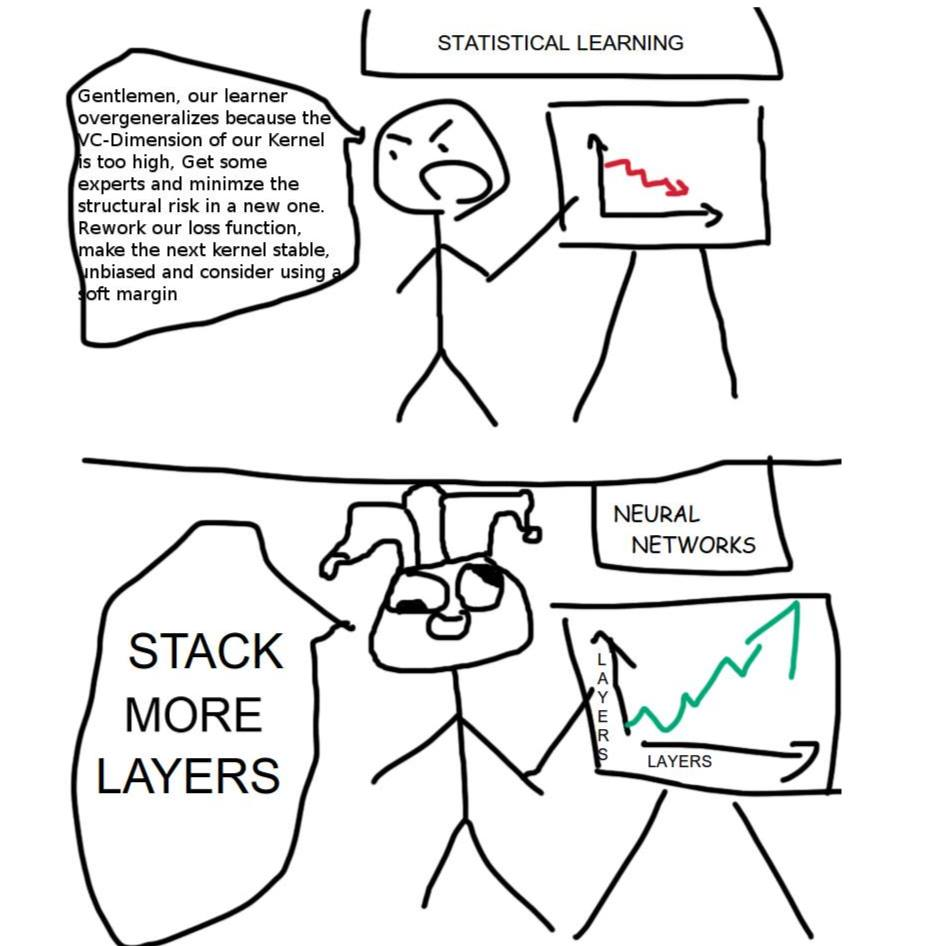
\includegraphics[width=0.4\textwidth]{Figures/shine_figures/more_layers.jpg}\caption{Credits: \href{reddit.com/r/ProgrammerHumor/comments/5si1f0/machine_learning_approaches/}{reddit.com/r/ProgrammerHumor/comments/5si1f0/machine\_learning\_approaches/}}
            \onslide<3>\centering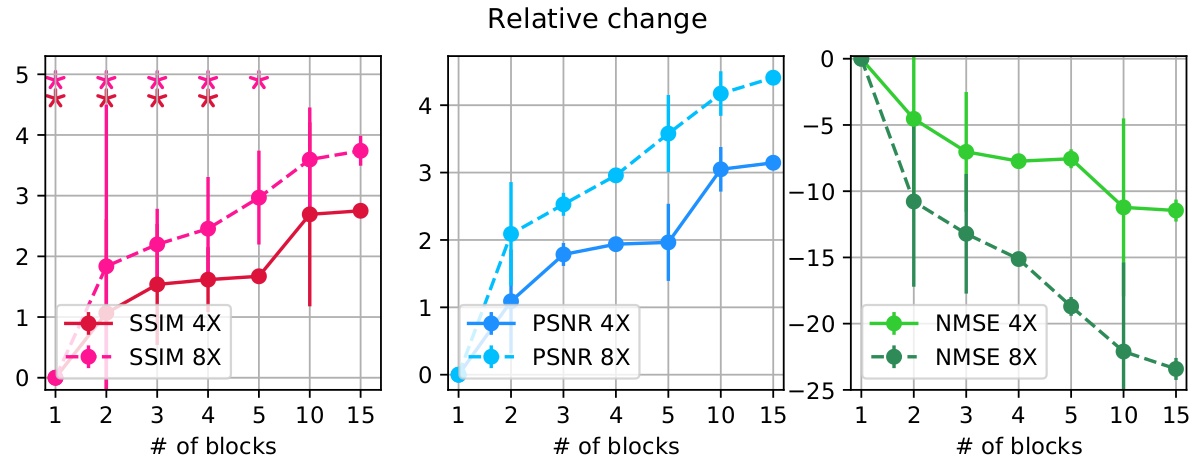
\includegraphics[width=0.78\textwidth]{Figures/shine_figures/pezzotti.png}\caption{\textbf{Performance of an unrolled MRI reconstruction network function of the number of iteration units (blocks).}\footfullcite{Pezzotti2020AnReconstruction}}
        \end{overprint}
    \end{figure}
\end{frame}

\begin{frame}{Can we go deeper?}
    % in the current state not: activations + constrained memory
    The big problem at hand is that deeper models need more memory to train, and the memory we have is constrained.
    \pause

    This memory requirement comes primarily from the activations of the model, not from the model weights.
    \pause

    \begin{center}
        \begin{tikzpicture}[
            font=\Large, node distance=5em,>=stealth,
            highlight/.style={rounded rectangle, draw=red!67, dashed, inner sep=0.1em},
        ]
            % nodes
            \node (input) {$\ldots$};
            \node (op) [rounded rectangle, right=of input, draw=black!87] {$\exp^{\thetab^\top \cdot}$};
            \node (output) [right=of op] {$\ldots$};
            \node (op_params) [below=of op] {$\thetab$};
            % arrows
            %% input to op
            \draw[->] (input.east) -- node [midway,below] {$\xb$} node [midway,above, visible on=<5->] {
                $\frac{\partial \mathcal{L}}{\partial \xb}$\alt<6->{\hspace{-0.5em}
                    \alt<7->{
                        $= \frac{\partial \mathcal{L}}{\partial \yb} \tikzmarknode[highlight]{y_x}{\yb} . \thetab $
                    }{
                        $= \frac{\partial \mathcal{L}}{\partial \yb} \frac{\partial \yb}{\partial \xb}$
                    }
                }{ ?}
            } (op.west);
            %% op to output
            \draw[->] (op) -- node (y) [midway,below] {$\alt<7->{\tikzmarknode[highlight]{y}{\yb}}{\yb}$} node [midway,above, visible on=<4->] {$\hookleftarrow \frac{\partial \mathcal{L}}{\partial \yb}$}  (output);
            %% op to op_params
            \draw[line width=0.1em] (op.south) -- node [midway, right, visible on=<5->] {
                $\frac{\partial \mathcal{L}}{\partial \thetab}$ \alt<6->{\hspace{-0.5em}
                    \alt<7->{
                        $= \frac{\partial \mathcal{L}}{\partial \yb} \tikzmarknode[highlight]{y_theta}{\yb} . \xb $
                    }{
                        $= \frac{\partial \mathcal{L}}{\partial \yb} \frac{\partial \yb}{\partial \thetab}$
                    }
                }{?}
            } (op_params.north);
        \end{tikzpicture}    
    \end{center}
    
\end{frame}

\begin{frame}{The modeling solutions}
    % gradient checkpointing
    % Invertible networks
    % Implicit models
    On the modeling side, several solutions exist:
    \begin{itemize}[<+->]
        \item Gradient checkpointing~\citep{Chen2016TrainingCost}
        \item Invertible networks~\citep{Gomez2017TheActivations,Sander2021MomentumNetworks}
        \item Implicit models~\citep{Chen2018NeuralEquations,Bai2019DeepModels}
    \end{itemize}
\end{frame}

\begin{frame}{Deep Equilibrium networks}
    % give equation and how to compute the gradient with IFT
\end{frame}

\subsection{SHINE}
\begin{frame}{The limits of DEQs}
    % they are slow to train
\end{frame}

\begin{frame}{Why are DEQs slow?}
    % bc of Jacobian inversion
\end{frame}

\begin{frame}{Can we avoid the Jacobian inversion?}
    % yes: reuse a by-product of the forward pass, share the inverse estimate
\end{frame}

\begin{frame}{Application to Hyperparameter optimization}
    % it's also a bilevel prob
\end{frame}

\begin{frame}{Results on DEQs}

\end{frame}